\section{Auswertung}
\label{sec:Auswertung}

Im Folgenden werden die aufgenommenen Messreihen ausgewertet, um die Evakuierungskurven sowie das effektive Saugvermögen beider Pumpentypen zu bestimmen. Das effektive Saugvermögen wird sowohl anhand der Evakuierungskurven, als auch anhand der Leckratenmessungen bestimmt. Scans der Originalmessdaten sind im Anhang zu finden.

\subsection{Fehlerrechnung}
\noindent
Wenn mehrere voneinander unabhängige fehlerbehaftete Größen miteinander verrechnet werden, wird die Gaußsche Fehlerfortpflanzung
\begin{equation}
\Delta f = \sqrt{\sum_{i \, = \, 1}^{n} \, \left(\frac{\partial f}{\partial x_i} \, \Delta x_i\right)^2}
\label{eq:ffp}
\end{equation}
genutzt, um den Fehler der berechneten Größe zu bestimmen.\\
Bei der Mittelwertbildung der Messgrößen aus den Messreihen ist zu beachten, dass die Unsicherheit $\Delta p$ des arithmetischen Mittelwerts $\bar{p}$ einer Observablen $p$ bei $n$ unabhängigen Messungen nach
\begin{equation}
\Delta p =  \sqrt{\frac{1}{n(n-1)} \sum_{i \, = \, 1}^{n} \, \left(\bar{p}- p_i\right)^2}
\label{eq:mittel}
\end{equation}
berechnet wird. Bei den unterschiedlichen Pumpentypen werden verschiedene Messgeräte genutzt, die zu unterschiedlichen Messungenauigkeiten für die einzelnen Messwerte führen, welche in den jeweiligen Unterabschnitten betrachtet werden.

%.......
\noindent
Die Fehlerfortpflanzung der Saugleistung bestimmt sich also zu
\begin{equation*}
  \sigma_{S} = \sqrt{\left(\frac{m^2}{p_g^2}\right) \cdot \sigma_{V}^2 + \left(\frac{V^2}{p_g^2}\right) \cdot \sigma_m^2 + \left(\frac{m^2 V^2}{p_g^4}\right) \cdot \sigma_p^2} \quad .
\end{equation*}


\subsection{Turbopumpe}
Als Messgerät bei den Messungen an der Turbopumpe wurde das PKR 360, Pfeiffer Vacuum Messgerät (kombinierter Pirani/Kaltkathode-Sensor) verwendet. Die Messungenauigkeit des genutzten Messgeräts beträgt 30\% im Bereich von  $\SI{1e-8}{\milli\bar}$ bis $\SI{100}{\milli\bar}$ und 50\% im Bereich von $\SI{100}{\milli\bar}$ bis $\SI{1000}{\milli\bar}$ \cite{V70}.

\subsubsection{Evakuierungskurve}
Für die Evakuierungsmessung der Turbopumpe wird über 120 Sekunden der Druck alle 10 Sekunden gemessen, innerhalb der ersten 20 Sekunden sogar alle 5 Sekunden. Auf diese Weise werden 3 Messreihen aufgenommen. In \autoref{tab:table} sind die Ergebnisse dieser Messreihen mit den jeweiligen Fehlern aufgelistet. Für den Mittelwert des Drucks wurde zusätzlich der Fehler des Mittelwerts (\autoref{eq:mittel}) berechnet. 



\begin{table}[H]
  \centering
  \caption{Messreihen zur Evakuierungsmessung der Turbopumpe}
  \label{tab:table}
  \begin{tabular}{rllll}
    \hline
       t [s] & p1 [mbar]         & p2 [mbar]         & p3 [mbar]         &$\bar{p}$ [mbar]                   \\
    \hline
           0 & 0.0050 \pm 0.0015   & 0.0050 \pm 0.0015   & 0.0050 \pm 0.0015   & 0.0050 \pm 0.0015   \\
           5 & 0.00032 \pm 0.00010 & 0.00039 \pm 0.00012 & 0.00038 \pm 0.00011 & 0.00036 \pm 0.00011 \\
          10 & 0.00012 \pm 0.00004 & 0.00013 \pm 0.00004 & 0.00012 \pm 0.00004 & 0.00012 \pm 0.00004 \\
          15 & (5.7 \pm 1.7)$*10^{-5}$   & (5.7 \pm 1.7)$*10^{-5}$   & (6.0 \pm 1.8)$*10^{-5}$   & (5.8 \pm 1.7)$*10^{-5}$   \\
          20 & (4.1 \pm 1.2)$*10^{-5}$   & (4.1 \pm 1.2)$*10^{-5}$   & (4.2 \pm 1.3)$*10^{-5}$   & (4.1 \pm 1.2)$*10^{-5}$   \\
          30 & (3.0 \pm 0.9)$*10^{-5}$   & (3.2 \pm 1.0)$*10^{-5}$   & (3.2 \pm 1.0)$*10^{-5}$   & (3.1 \pm 0.9)$*10^{-5}$   \\
          40 & (2.8 \pm 0.8)$*10^{-5}$   & (2.8 \pm 0.9)$*10^{-5}$   & (2.9 \pm 0.9)$*10^{-5}$   & (2.8 \pm 0.8)$*10^{-5}$   \\
          50 & (2.6 \pm 0.8)$*10^{-5}$   & (2.6 \pm 0.8)$*10^{-5}$   & (2.6 \pm 0.8)$*10^{-5}$   & (2.6 \pm 0.8)$*10^{-5}$   \\
          60 & (2.4 \pm 0.7)$*10^{-5}$   & (2.5 \pm 0.7)$*10^{-5}$   & (2.5 \pm 0.8)$*10^{-5}$   & (2.5 \pm 0.7)$*10^{-5}$   \\
          70 & (2.3 \pm 0.7)$*10^{-5}$   & (2.4 \pm 0.7)$*10^{-5}$   & (2.4 \pm 0.7)$*10^{-5}$   & (2.4 \pm 0.7)$*10^{-5}$   \\
          80 & (2.3 \pm 0.7)$*10^{-5}$   & (2.3 \pm 0.7)$*10^{-5}$   & (2.3 \pm 0.7)$*10^{-5}$   & (2.3 \pm 0.7)$*10^{-5}$   \\
          90 & (2.2 \pm 0.7)$*10^{-5}$   & (2.2 \pm 0.7)$*10^{-5}$   & (2.2 \pm 0.7)$*10^{-5}$   & (2.2 \pm 0.7)$*10^{-5}$   \\
         100 & (2.1 \pm 0.6)$*10^{-5}$   & (2.2 \pm 0.6)$*10^{-5}$   & (2.2 \pm 0.7)$*10^{-5}$   & (2.2 \pm 0.6)$*10^{-5}$   \\
         110 & (2.1 \pm 0.6)$*10^{-5}$   & (2.1 \pm 0.6)$*10^{-5}$   & (2.1 \pm 0.6)$*10^{-5}$   & (2.1 \pm 0.6)$*10^{-5}$   \\
         120 & (2.1 \pm 0.6)$*10^{-5}$   & (2.1 \pm 0.6)$*10^{-5}$   & (2.1 \pm 0.6)$*10^{-5}$   & (2.1 \pm 0.6)$*10^{-5}$   \\
    \hline
    \end{tabular}
  \end{table}
\noindent
  Um die Messwerte an eine Gerade der Form \begin{equation}
    y = m \cdot x + n
    \label{eqn:lin}
  \end{equation}
  \noindent
  angleichen zu können, müssen sie über den Zusammenhang 
  \begin{equation}
    \ln\left(\frac{p(t) - p_{end}}{p_0 - p_{end}}\right)
  \end{equation} 
  \noindent
  linearisiert werden. 
  Für die Fehlerfortpflanzung der logarithmierten Werte wurde die Formel 
  \begin{equation*}
    \sigma = \sqrt{\frac{\sigma_p^2}{(p-p_E)^2}+\frac{\sigma_{p0}^2}{(p_0-p_E)^2}+\sigma_{p_E}^2 \left(\frac{1}{p_0-p_E}-\frac{1}{p-p_E}\right)^2}
  \end{equation*}
  genutzt, die aus der Gaußschen Fehlerfortpflanzung (\autoref{eq:ffp}) resultiert. Die logarithmierten Werte sind in \autoref{tab:logtable} aufgelistet (gemessen wurden $p_0 = 5*10^{-3}$ und $p_E = 1.5*10^{-5}$).\\

  \begin{table}[H]
    \centering
    \caption{Logarithmierte Messreihen zur Evakuierungsmessung der Turbopumpe}
    \label{tab:logtable}
    \begin{tabular}{rl}
      \hline
         t [s] & $\ln(\frac{p-p_{E}}{p_{0}-p_{E}})$ \\
      \hline
             0 & 0.0 \pm 0.4  \\
             5 & -2.7 \pm 0.4 \\
            10 & -3.8 \pm 0.5 \\
            15 & -4.8 \pm 0.5 \\
            20 & -5.2 \pm 0.6 \\
            30 & -5.7 \pm 0.7 \\
            40 & -5.9 \pm 0.8 \\
            50 & -6.1 \pm 0.9 \\
            60 & -6.2 \pm 0.9 \\
            70 & -6.3 \pm 1.0 \\
            80 & -6.5 \pm 1.1 \\
            90 & -6.5 \pm 1.2 \\
           100 & -6.6 \pm 1.2 \\
           110 & -6.7 \pm 1.3 \\
           120 & -6.7 \pm 1.3 \\
      \hline
      \end{tabular}
    \end{table}

\noindent
Da die Saugleistung der Pumpe nicht für den gesamten Druckbereich konstant ist, wird die lineare Ausgleichsrechnung für drei unterschiedliche Druckbereiche durchgeführt.
Die logarithmierten Werte mit Ausgleichsgeraden für die 3 Druckbereiche sind in \autoref{fig:plot} graphisch dargestellt.

\begin{figure}[H]
  \centering
  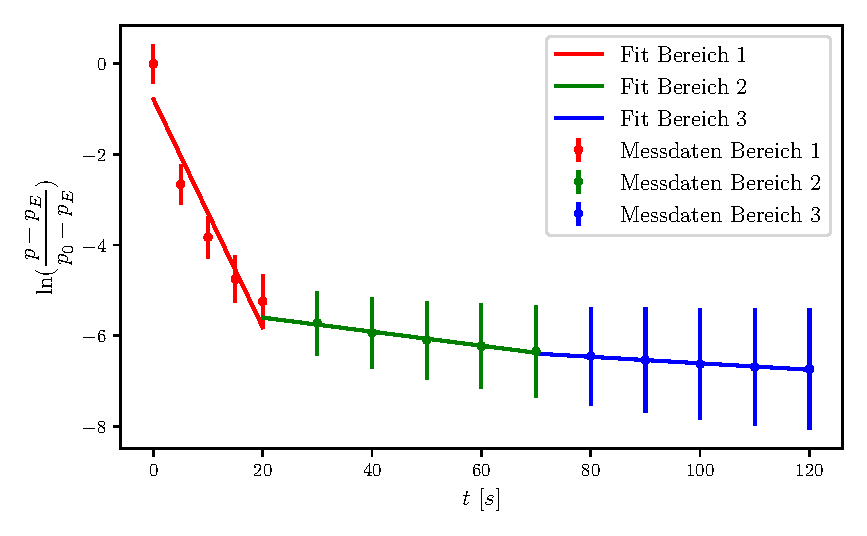
\includegraphics{build/plots/plot_ev_turbo.pdf}
  \caption{Logarithmierte Werte mit Ausgleichsgeraden für 3 Druckbereiche zur Evakuierungsmessung der Turbopumpe}
  \label{fig:plot}
\end{figure}
\noindent
Aus den Parametern der Ausgleichsrechnung lässt sich über $ S = -mV $ die Saugvermögen bestimmen. Diese Parameter sowie das Saugvermögen sind in der folgenden Tabelle für die entsprechenden Druckbereiche aufgelistet.

\begin{table}[H]
  \centering
  \small
  \label{tab:parat}
  \begin{tabular}{l  c c c}
   \toprule
   {Druckbereich} & $\text{m} [\si{\per\second}]$ & $\text{n}$ & $\text{S} [\si{\litre\per\second}]$ \\
   \midrule
   $\SI{5e-3}{\milli\bar}$ bis $\SI{4.2e-5}{\milli\bar}$ & -0.2516 \pm 0.04681 & -0.7815 \pm 0.04681 & 8.3019 \pm 1.75376\\
   $\SI{4.2e-5}{\milli\bar}$ bis $\SI{2.35e-5}{\milli\bar}$ &-0.0155 \pm 0.00109 & -5.2908 \pm 0.00109 & 0.5115 \pm 0.06254\\
   $\SI{2.35e-5}{\milli\bar}$ bis $\SI{2.1e-5}{\milli\bar}$ & -0.0071 \pm 0.00057  & -5.8948 \pm 0.00057 & 0.2355 \pm 0.03007\\
  \bottomrule
  \end{tabular}
  \caption{Parameter der Ausgleichsgeraden und Ergebnisse für das Saugvermögen.}
\end{table} 

\subsubsection{Leckratenmessungen}
Bei den Leckratenmessungen für die Turbopumpe wird, nachdem jeweils ein bestimmter Gleichgewichtsdruck eingestellt wurde, über einen Zeitraum von $\SI{120}{\second}$ alle $\SI{10}{\second}$ der Druck aufgenommen. Zu diesen Werten wird dann wieder eine lineare Ausgleichsrechnung (zur Gerade, \autoref{eqn:lin}) durchgeführt. Die Messungen wurden bei den Gleichgewichtsdrücken $p_g = \SI{1e-4}{\milli\bar}$(siehe \autoref{tab:table1} und \autoref{fig:plott1}), $p_g = \SI{2e-4}{\milli\bar}$(siehe \autoref{tab:table2} und \autoref{fig:plott2}), $p_g = \SI{5e-5}{\milli\bar}$(siehe \autoref{tab:table3} und \autoref{fig:plott3}) und $p_g = \SI{7e-5}{\milli\bar}$(siehe \autoref{tab:table4} und \autoref{fig:plott4}) durchgeführt.

\begin{table}[H]
  \centering
  \caption{Messreihen zur Leckratenmessung der Turbopumpe mit $p_g = 1*10^{-4}$ mbar}
  \label{tab:table1}
  \begin{tabular}{rllll}
    \hline
       t [s] & p1 [mbar]         & p2 [mbar]         & p3 [mbar]         & $\bar{p}$ [mbar]     \\
    \hline
          10 & 0.00027 \pm 0.00008 & 0.00027 \pm 0.00008 & 0.00028 \pm 0.00008 & 0.00027 \pm 0.00008 \\
          20 & 0.00042 \pm 0.00013 & 0.00042 \pm 0.00012 & 0.00042 \pm 0.00013 & 0.00042 \pm 0.00013 \\
          30 & 0.00055 \pm 0.00016 & 0.00055 \pm 0.00017 & 0.00056 \pm 0.00017 & 0.00055 \pm 0.00017 \\
          40 & 0.00067 \pm 0.00020 & 0.00067 \pm 0.00020 & 0.00068 \pm 0.00020 & 0.00067 \pm 0.00020 \\
          50 & 0.00081 \pm 0.00024 & 0.00081 \pm 0.00024 & 0.00083 \pm 0.00025 & 0.00082 \pm 0.00024 \\
          60 & 0.00098 \pm 0.00029 & 0.00096 \pm 0.00029 & 0.00097 \pm 0.00029 & 0.00097 \pm 0.00029 \\
          70 & 0.00111 \pm 0.00033 & 0.00110 \pm 0.00033 & 0.00111 \pm 0.00033 & 0.00111 \pm 0.00033 \\
          80 & 0.0013 \pm 0.0004   & 0.0013 \pm 0.0004   & 0.0013 \pm 0.0004   & 0.0013 \pm 0.0004   \\
          90 & 0.0015 \pm 0.0004   & 0.0015 \pm 0.0004   & 0.0015 \pm 0.0005   & 0.0015 \pm 0.0005   \\
         100 & 0.0017 \pm 0.0005   & 0.0017 \pm 0.0005   & 0.0017 \pm 0.0005   & 0.0017 \pm 0.0005   \\
         110 & 0.0019 \pm 0.0006   & 0.0019 \pm 0.0006   & 0.0019 \pm 0.0006   & 0.0019 \pm 0.0006   \\
         120 & 0.0021 \pm 0.0006   & 0.0021 \pm 0.0006   & 0.0021 \pm 0.0006   & 0.0021 \pm 0.0006   \\
    \hline
    \end{tabular}
  \end{table}

  \begin{figure}[H]
    \centering
    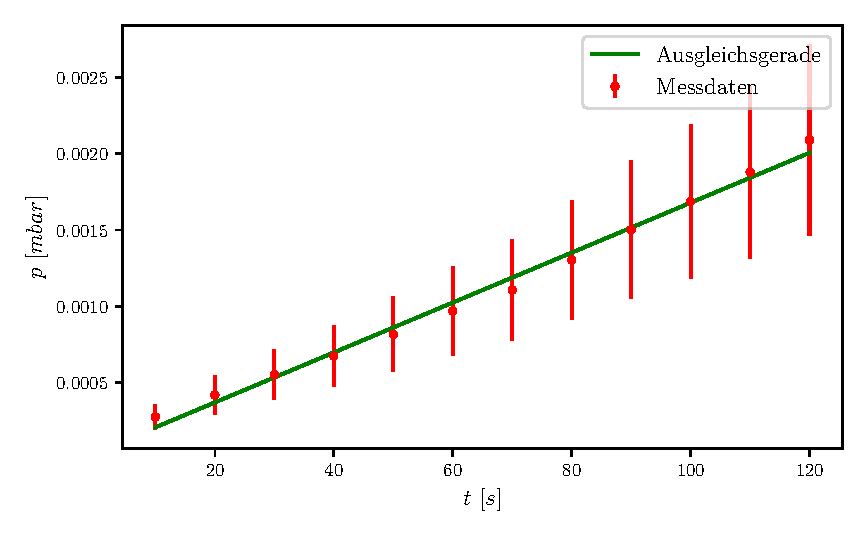
\includegraphics{build/plots/leck_turbo_0.0001.pdf}
    \caption{Messwerte mit Ausgleichsgerade zur Leckratenmessung der Turbopumpe bei $p_g = 1*10^{-4}$ mbar}
    \label{fig:plott1}
  \end{figure}

  \begin{table}[H]
    \centering
    \caption{Messreihen zur Leckratenmessung der Turbopumpe mit $p_g = 2*10^{-4}$ mbar}
    \label{tab:table2}
    \begin{tabular}{rllll}
      \hline
         t [s] & p1 [mbar]         & p2 [mbar]         & p3 [mbar]         & $\bar{p}$ [mbar]     \\
      \hline
            10 & 0.00054 \pm 0.00016 & 0.00052 \pm 0.00016 & 0.00053 \pm 0.00016 & 0.00053 \pm 0.00016 \\
            20 & 0.00084 \pm 0.00025 & 0.00083 \pm 0.00025 & 0.00082 \pm 0.00025 & 0.00083 \pm 0.00025 \\
            30 & 0.0012 \pm 0.0004   & 0.0012 \pm 0.0004   & 0.00116 \pm 0.00035 & 0.00118 \pm 0.00035 \\
            40 & 0.0016 \pm 0.0005   & 0.0016 \pm 0.0005   & 0.0016 \pm 0.0005   & 0.0016 \pm 0.0005   \\
            50 & 0.0021 \pm 0.0006   & 0.0021 \pm 0.0006   & 0.0021 \pm 0.0006   & 0.0021 \pm 0.0006   \\
            60 & 0.0027 \pm 0.0008   & 0.0026 \pm 0.0008   & 0.0026 \pm 0.0008   & 0.0026 \pm 0.0008   \\
            70 & 0.0032 \pm 0.0010   & 0.0032 \pm 0.0009   & 0.0031 \pm 0.0009   & 0.0032 \pm 0.0009   \\
            80 & 0.0038 \pm 0.0011   & 0.0038 \pm 0.0011   & 0.0037 \pm 0.0011   & 0.0038 \pm 0.0011   \\
            90 & 0.0044 \pm 0.0013   & 0.0043 \pm 0.0013   & 0.0043 \pm 0.0013   & 0.0043 \pm 0.0013   \\
           100 & 0.0050 \pm 0.0015   & 0.0050 \pm 0.0015   & 0.0050 \pm 0.0015   & 0.0050 \pm 0.0015   \\
           110 & 0.0057 \pm 0.0017   & 0.0057 \pm 0.0017   & 0.0056 \pm 0.0017   & 0.0057 \pm 0.0017   \\
           120 & 0.0063 \pm 0.0019   & 0.0063 \pm 0.0019   & 0.0062 \pm 0.0019   & 0.0063 \pm 0.0019   \\
      \hline
      \end{tabular}
    \end{table}

    \begin{figure}[H]
      \centering
      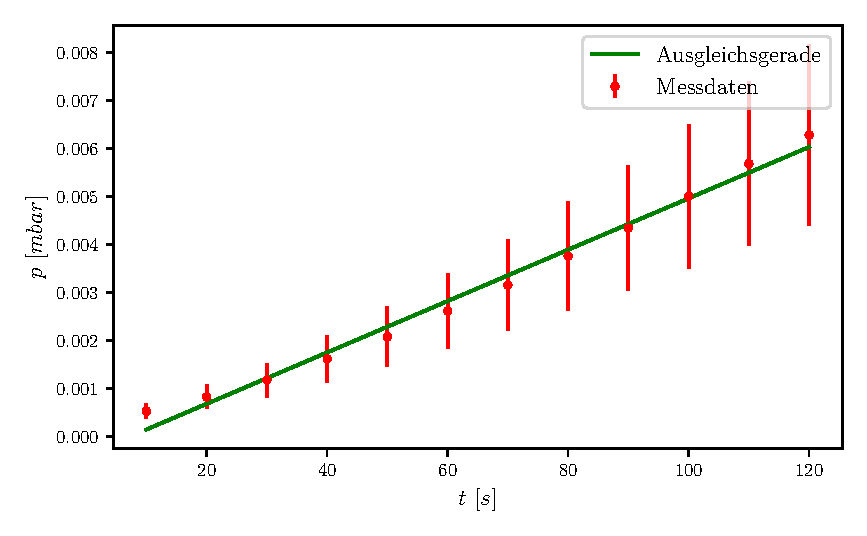
\includegraphics{build/plots/leck_turbo_0.0002.pdf}
      \caption{Messwerte mit Ausgleichsgerade zur Leckratenmessung der Turbopumpe bei $p_g = 2*10^{-4}$ mbar}
      \label{fig:plott2}
    \end{figure}

    \begin{table}[H]
      \centering
      \caption{Messreihen zur Leckratenmessung der Turbopumpe mit $p_g = 5*10^{-5}$ mbar}
      \label{tab:table3}
      \begin{tabular}{rllll}
        \hline
           t [s] & p1 [mbar]         & p2 [mbar]         & p3 [mbar]         & $\bar{p}$ [mbar]     \\
        \hline
              10 & 0.00014 \pm 0.00004 & 0.00014 \pm 0.00004 & 0.00014 \pm 0.00004 & 0.00014 \pm 0.00004 \\
              20 & 0.00021 \pm 0.00006 & 0.00021 \pm 0.00006 & 0.00021 \pm 0.00006 & 0.00021 \pm 0.00006 \\
              30 & 0.00028 \pm 0.00008 & 0.00028 \pm 0.00008 & 0.00028 \pm 0.00008 & 0.00028 \pm 0.00008 \\
              40 & 0.00034 \pm 0.00010 & 0.00034 \pm 0.00010 & 0.00034 \pm 0.00010 & 0.00034 \pm 0.00010 \\
              50 & 0.00039 \pm 0.00012 & 0.00040 \pm 0.00012 & 0.00040 \pm 0.00012 & 0.00040 \pm 0.00012 \\
              60 & 0.00045 \pm 0.00013 & 0.00046 \pm 0.00014 & 0.00045 \pm 0.00014 & 0.00045 \pm 0.00014 \\
              70 & 0.00051 \pm 0.00015 & 0.00051 \pm 0.00015 & 0.00052 \pm 0.00015 & 0.00051 \pm 0.00015 \\
              80 & 0.00056 \pm 0.00017 & 0.00056 \pm 0.00017 & 0.00057 \pm 0.00017 & 0.00056 \pm 0.00017 \\
              90 & 0.00061 \pm 0.00018 & 0.00062 \pm 0.00019 & 0.00062 \pm 0.00019 & 0.00062 \pm 0.00019 \\
             100 & 0.00066 \pm 0.00020 & 0.00067 \pm 0.00020 & 0.00066 \pm 0.00020 & 0.00066 \pm 0.00020 \\
             110 & 0.00072 \pm 0.00022 & 0.00072 \pm 0.00022 & 0.00072 \pm 0.00022 & 0.00072 \pm 0.00022 \\
             120 & 0.00078 \pm 0.00023 & 0.00079 \pm 0.00024 & 0.00078 \pm 0.00024 & 0.00079 \pm 0.00024 \\
        \hline
        \end{tabular}
      \end{table}
    
      \begin{figure}[H]
        \centering
        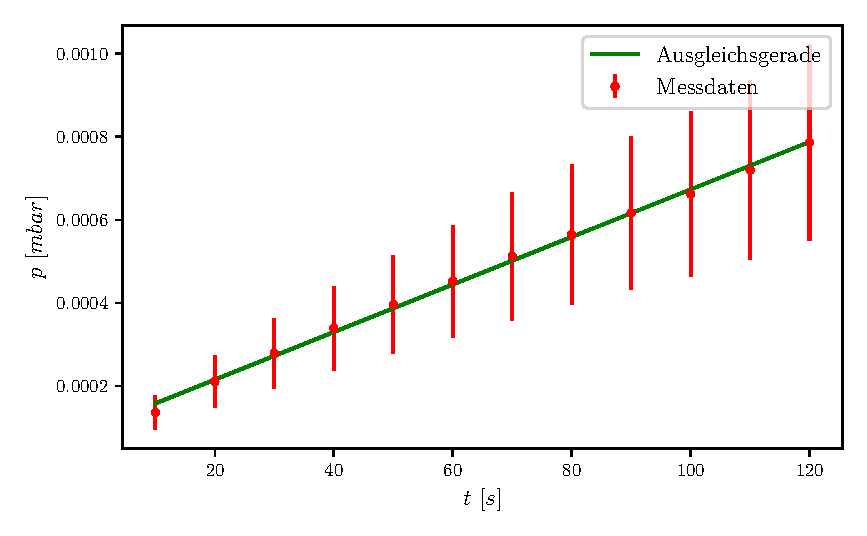
\includegraphics{build/plots/leck_turbo_5e-05.pdf}
        \caption{Messwerte mit Ausgleichsgerade zur Leckratenmessung der Turbopumpe bei $p_g = 5*10^{-5}$ mbar}
        \label{fig:plott3}
      \end{figure}

      \begin{table}[H]
        \centering
        \caption{Messreihen zur Leckratenmessung der Turbopumpe mit $p_g = 7*10^{-5}$ mbar}
        \label{tab:table4}
        \begin{tabular}{rllll}
          \hline
             t [s] & p1 [mbar]         & p2 [mbar]         & p3 [mbar]         & $\bar{p}$ [mbar]     \\
          \hline
                10 & 0.00020 \pm 0.00006 & 0.00020 \pm 0.00006 & 0.00019 \pm 0.00006 & 0.00020 \pm 0.00006 \\
                20 & 0.00030 \pm 0.00009 & 0.00030 \pm 0.00009 & 0.00029 \pm 0.00009 & 0.00030 \pm 0.00009 \\
                30 & 0.00040 \pm 0.00012 & 0.00040 \pm 0.00012 & 0.00040 \pm 0.00012 & 0.00040 \pm 0.00012 \\
                40 & 0.00049 \pm 0.00015 & 0.00049 \pm 0.00015 & 0.00049 \pm 0.00015 & 0.00049 \pm 0.00015 \\
                50 & 0.00057 \pm 0.00017 & 0.00058 \pm 0.00017 & 0.00058 \pm 0.00017 & 0.00058 \pm 0.00017 \\
                60 & 0.00065 \pm 0.00020 & 0.00066 \pm 0.00020 & 0.00066 \pm 0.00020 & 0.00066 \pm 0.00020 \\
                70 & 0.00075 \pm 0.00022 & 0.00075 \pm 0.00022 & 0.00075 \pm 0.00022 & 0.00075 \pm 0.00022 \\
                80 & 0.00084 \pm 0.00025 & 0.00084 \pm 0.00025 & 0.00084 \pm 0.00025 & 0.00084 \pm 0.00025 \\
                90 & 0.00096 \pm 0.00029 & 0.00095 \pm 0.00028 & 0.00095 \pm 0.00028 & 0.00095 \pm 0.00029 \\
               100 & 0.00109 \pm 0.00033 & 0.00107 \pm 0.00032 & 0.00107 \pm 0.00032 & 0.00108 \pm 0.00032 \\
               110 & 0.00116 \pm 0.00035 & 0.00116 \pm 0.00035 & 0.00115 \pm 0.00034 & 0.00116 \pm 0.00035 \\
               120 & 0.0013 \pm 0.0004   & 0.0013 \pm 0.0004   & 0.0013 \pm 0.0004   & 0.0013 \pm 0.0004   \\
          \hline
          \end{tabular}
        \end{table}
      
        \begin{figure}[H]
          \centering
          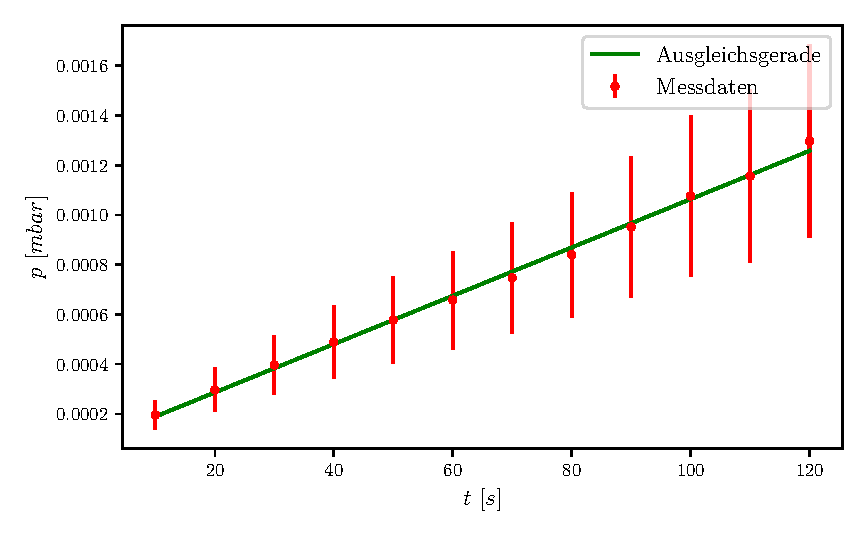
\includegraphics{build/plots/leck_turbo_7.000000000000001e-05.pdf}
          \caption{Messwerte mit Ausgleichsgerade zur Leckratenmessung der Turbopumpe bei $p_g = 7*10^{-5}$ mbar}
          \label{fig:plott4}
        \end{figure}
\noindent
Schließlich können wieder die Parameter der Ausgleichsgeraden und das Saugvermögen über $S = \frac{-V}{p_g}\cdot m$ bestimmt werden. Die Parameter und das entsprechende Saugvermögen für die jeweiligen Gleichgewichtsdrücke sind im Folgenden tabellarisch aufgelistet. 
        \begin{table}[H]
          \centering
          \small
          \label{tab:para_leck_turbo}
          \begin{tabular}{l  c c c}
           \toprule
           $p_g [\si{\milli\bar}]$ & $\text{m} [\si{\per\second}]$ & $\text{n}$ & $\text{S} [\si{\litre\per\second}]$ \\
           \midrule
           $\SI{1e-4}{\milli\bar}$ & 0.00001637 \pm 0.00000046 & 0.00004194 \pm 0.00000046 & 5.4027 \pm 0.56130\\
           $\SI{2e-4}{\milli\bar}$ & 0.00005350 \pm 0.00000175 & -0.00038608 \pm 0.00000175 & 8.8272 \pm 0.92869\\
           $\SI{5e-5}{\milli\bar}$ & 0.00000573 \pm 0.00000009  & 0.00010065 \pm 0.00000009 & 3.7791 \pm 0.38249\\
           $\SI{7e-5}{\milli\bar}$ & 0.00000972 \pm 0.00000017  & 0.00009193 \pm 0.00000017 & 4.5814 \pm 0.46502\\
          \bottomrule
          \end{tabular}
          \caption{Parameter der Ausgleichsgeraden und Ergebnisse für das Saugvermögen zur Leckratenmessung der Turbopumpe für unterschiedliche Gleichgewichtsdrücke}
        \end{table} 

\subsection{Drehschieberpumpe}
Für die Messungen mit der Drehschieberpumpe wird als Fehler für Druckwerte kleiner als $\SI{2e-3}{\milli\bar}$ ein Faktor $2$ vom Messwert, für $\SI{2e-3}{\milli\bar}$ bis $\SI{10}{\milli\bar}$ der Wert $\pm\; \SI{120}{\milli\bar}$ 
und für $\SI{10}{\milli\bar}$ bis $\SI{1200}{\milli\bar}$ der Wert $\pm \;\SI{3.6}{\milli\bar}$ als Messfehler genutzt\cite{V70}. \\\\
\subsubsection{Evakuierungskurve}
Bei dieser Messung wurden über einen Zeitraum von $\SI{600}{\second}$ alle $\SI{10}{\second}$ Druckwerte aufgenommen.
Das Vorgehen für die Auswertung der Evakuierungsmessung erfolgt ansonsten analog zum Vorgehen bei der Turbopumpe.  
Als Startdruck wurde $p_0 = \SI{998}{\milli\bar}$ und als Enddruck wurde $p_E = \SI{0.012}{\milli\bar}$ gemessen.
\begin{table}{H}
  \centering
  \caption{Messreihen zur Evakuierungsmessung der Drehschieberpumpe (Bereich bis 300 s)}
  \label{tab:dreh}
  \begin{tabular}{rllll}
    \hline
       t [s] & p1 [mbar]     & p2 [mbar]     & p3 [mbar]     & $\bar{p}$ [mbar]               \\
    \hline
           0 & 998 \pm 4       & 998 \pm 4       & 998 \pm 4       & 998 \pm 4       \\
          10 & 652 \pm 4       & 646 \pm 4       & 654 \pm 4       & 651 \pm 4       \\
          20 & 487 \pm 4       & 482 \pm 4       & 481 \pm 4       & 483 \pm 4       \\
          30 & 352 \pm 4       & 359 \pm 4       & 361 \pm 4       & 357 \pm 4       \\
          40 & 262 \pm 4       & 268 \pm 4       & 269 \pm 4       & 266 \pm 4       \\
          50 & 200 \pm 4       & 197 \pm 4       & 198 \pm 4       & 198 \pm 4       \\
          60 & 145 \pm 4       & 144 \pm 4       & 145 \pm 4       & 145 \pm 4       \\
          70 & 106 \pm 4       & 105 \pm 4       & 106 \pm 4       & 106 \pm 4       \\
          80 & 78 \pm 4        & 77 \pm 4        & 78 \pm 4        & 78 \pm 4        \\
          90 & 57 \pm 4        & 56 \pm 4        & 57 \pm 4        & 57 \pm 4        \\
         100 & 41 \pm 4        & 41 \pm 4        & 41 \pm 4        & 41 \pm 4        \\
         110 & 30 \pm 4        & 30 \pm 4        & 3.00 \pm 0.30   & 21 \pm 4        \\
         120 & 22 \pm 4        & 22 \pm 4        & 3.10 \pm 0.31   & 15 \pm 4        \\
         130 & 15 \pm 4        & 16 \pm 4        & 16 \pm 4        & 16 \pm 4        \\
         140 & 12 \pm 4        & 12 \pm 4        & 12 \pm 4        & 12 \pm 4        \\
         150 & 8.5 \pm 0.9     & 8.4 \pm 0.8     & 8.4 \pm 0.8     & 8.4 \pm 0.8     \\
         160 & 6.2 \pm 0.6     & 6.2 \pm 0.6     & 6.2 \pm 0.6     & 6.2 \pm 0.6     \\
         170 & 4.6 \pm 0.5     & 4.5 \pm 0.5     & 4.6 \pm 0.5     & 4.6 \pm 0.5     \\
         180 & 3.6 \pm 0.4     & 3.6 \pm 0.4     & 3.6 \pm 0.4     & 3.6 \pm 0.4     \\
         190 & 2.90 \pm 0.29   & 2.80 \pm 0.28   & 2.90 \pm 0.29   & 2.87 \pm 0.29   \\
         200 & 2.30 \pm 0.23   & 2.30 \pm 0.23   & 2.30 \pm 0.23   & 2.30 \pm 0.23   \\
         210 & 1.90 \pm 0.19   & 1.90 \pm 0.19   & 1.90 \pm 0.19   & 1.90 \pm 0.19   \\
         220 & 1.60 \pm 0.16   & 1.60 \pm 0.16   & 1.70 \pm 0.17   & 1.63 \pm 0.16   \\
         230 & 1.40 \pm 0.14   & 1.40 \pm 0.14   & 1.40 \pm 0.14   & 1.40 \pm 0.14   \\
         240 & 1.20 \pm 0.12   & 1.20 \pm 0.12   & 1.20 \pm 0.12   & 1.20 \pm 0.12   \\
         250 & 1.10 \pm 0.11   & 1.10 \pm 0.11   & 1.10 \pm 0.11   & 1.10 \pm 0.11   \\
         260 & 0.93 \pm 0.09   & 0.94 \pm 0.09   & 0.95 \pm 0.10   & 0.94 \pm 0.09   \\
         270 & 0.84 \pm 0.08   & 0.86 \pm 0.09   & 0.86 \pm 0.09   & 0.85 \pm 0.09   \\
         280 & 0.76 \pm 0.08   & 0.77 \pm 0.08   & 0.77 \pm 0.08   & 0.77 \pm 0.08   \\
         290 & 0.69 \pm 0.07   & 0.70 \pm 0.07   & 0.69 \pm 0.07   & 0.69 \pm 0.07   \\
         300 & 0.64 \pm 0.06   & 0.64 \pm 0.06   & 0.64 \pm 0.06   & 0.64 \pm 0.06   \\
    \hline
    \end{tabular}
  \end{table}

  \begin{table}{H}
    \centering
    \caption{Messreihen zur Evakuierungsmessung der Drehschieberpumpe (Bereich 300 s bis 600 s)}
    \label{tab:dreh2}
    \begin{tabular}{rllll}
      \hline
         t [s] & p1 [mbar]     & p2 [mbar]     & p3 [mbar]     & $\bar{p}$ [mbar]               \\
      \hline
           300 & 0.64 \pm 0.06   & 0.64 \pm 0.06   & 0.64 \pm 0.06   & 0.64 \pm 0.06   \\
           310 & 0.60 \pm 0.06   & 0.60 \pm 0.06   & 0.60 \pm 0.06   & 0.60 \pm 0.06   \\
           320 & 0.55 \pm 0.06   & 0.55 \pm 0.06   & 0.56 \pm 0.06   & 0.55 \pm 0.06   \\
           330 & 0.52 \pm 0.05   & 0.51 \pm 0.05   & 0.52 \pm 0.05   & 0.52 \pm 0.05   \\
           340 & 0.48 \pm 0.05   & 0.48 \pm 0.05   & 0.48 \pm 0.05   & 0.48 \pm 0.05   \\
           350 & 0.45 \pm 0.05   & 0.45 \pm 0.05   & 0.45 \pm 0.05   & 0.45 \pm 0.05   \\
           360 & 0.42 \pm 0.04   & 0.40 \pm 0.04   & 0.40 \pm 0.04   & 0.41 \pm 0.04   \\
           370 & 0.40 \pm 0.04   & 0.38 \pm 0.04   & 0.37 \pm 0.04   & 0.38 \pm 0.04   \\
           380 & 0.38 \pm 0.04   & 0.36 \pm 0.04   & 0.350 \pm 0.035 & 0.36 \pm 0.04   \\
           390 & 0.36 \pm 0.04   & 0.340 \pm 0.034 & 0.340 \pm 0.034 & 0.347 \pm 0.035 \\
           400 & 0.330 \pm 0.033 & 0.340 \pm 0.034 & 0.330 \pm 0.033 & 0.333 \pm 0.033 \\
           410 & 0.320 \pm 0.032 & 0.310 \pm 0.031 & 0.320 \pm 0.032 & 0.317 \pm 0.032 \\
           420 & 0.320 \pm 0.032 & 0.310 \pm 0.031 & 0.320 \pm 0.032 & 0.317 \pm 0.032 \\
           430 & 0.310 \pm 0.031 & 0.310 \pm 0.031 & 0.310 \pm 0.031 & 0.310 \pm 0.031 \\
           440 & 0.300 \pm 0.030 & 0.290 \pm 0.029 & 0.300 \pm 0.030 & 0.297 \pm 0.030 \\
           450 & 0.280 \pm 0.028 & 0.280 \pm 0.028 & 0.280 \pm 0.028 & 0.280 \pm 0.028 \\
           460 & 0.260 \pm 0.026 & 0.270 \pm 0.027 & 0.270 \pm 0.027 & 0.267 \pm 0.027 \\
           470 & 0.250 \pm 0.025 & 0.260 \pm 0.026 & 0.260 \pm 0.026 & 0.257 \pm 0.026 \\
           480 & 0.240 \pm 0.024 & 0.250 \pm 0.025 & 0.250 \pm 0.025 & 0.247 \pm 0.025 \\
           490 & 0.230 \pm 0.023 & 0.230 \pm 0.023 & 0.130 \pm 0.013 & 0.197 \pm 0.020 \\
           500 & 0.220 \pm 0.022 & 0.220 \pm 0.022 & 0.220 \pm 0.022 & 0.220 \pm 0.022 \\
           510 & 0.210 \pm 0.021 & 0.210 \pm 0.021 & 0.210 \pm 0.021 & 0.210 \pm 0.021 \\
           520 & 0.210 \pm 0.021 & 0.200 \pm 0.020 & 0.200 \pm 0.020 & 0.203 \pm 0.020 \\
           530 & 0.190 \pm 0.019 & 0.190 \pm 0.019 & 0.200 \pm 0.020 & 0.193 \pm 0.019 \\
           540 & 0.180 \pm 0.018 & 0.180 \pm 0.018 & 0.190 \pm 0.019 & 0.183 \pm 0.018 \\
           550 & 0.180 \pm 0.018 & 0.180 \pm 0.018 & 0.190 \pm 0.019 & 0.183 \pm 0.018 \\
           560 & 0.170 \pm 0.017 & 0.170 \pm 0.017 & 0.180 \pm 0.018 & 0.173 \pm 0.017 \\
           570 & 0.170 \pm 0.017 & 0.170 \pm 0.017 & 0.170 \pm 0.017 & 0.170 \pm 0.017 \\
           580 & 0.160 \pm 0.016 & 0.160 \pm 0.016 & 0.160 \pm 0.016 & 0.160 \pm 0.016 \\
           590 & 0.160 \pm 0.016 & 0.150 \pm 0.015 & 0.160 \pm 0.016 & 0.157 \pm 0.016 \\
           600 & 0.150 \pm 0.015 & 0.150 \pm 0.015 & 0.150 \pm 0.015 & 0.150 \pm 0.015 \\
      \hline
      \end{tabular}
    \end{table}

  \begin{table}[H]
    \centering
    \caption{Logarithmierte Messreihen zur Evakuierungsmessung der Drehschieberpumpe}
    \label{tab:drehlog}
    \begin{tabular}{rlll}
      \hline
         t [s] & $\ln(\frac{p-p_{E}}{p_{0}-p_{E}})$ & t [s] & $\ln(\frac{p-p_{E}}{p_{0}-p_{E}})$ \\
         \hline
         0 & 0.000 \pm 0.005      & 310 & -7.44 \pm 0.10 \\
         10 & -0.428 \pm 0.007  & 320 & -7.52 \pm 0.10 \\
         20 & -0.725 \pm 0.008  & 330 & -7.59 \pm 0.10 \\
         30 & -1.027 \pm 0.011  & 340 & -7.67 \pm 0.10 \\
         40 & -1.321 \pm 0.014  & 350 & -7.73 \pm 0.10 \\
         50 & -1.616 \pm 0.019  & 360 & -7.84 \pm 0.10 \\
         60 & -1.931 \pm 0.025  & 370 & -7.90 \pm 0.10 \\
         70 & -2.246 \pm 0.034  & 380 & -7.95 \pm 0.10 \\
         80 & -2.55 \pm 0.05      & 390 & -8.00 \pm 0.10 \\
         90 & -2.87 \pm 0.06      & 400 & -8.04 \pm 0.10 \\
         100 & -3.19 \pm 0.09     & 410 & -8.09 \pm 0.10 \\
         110 & -3.86 \pm 0.17     & 420 & -8.09 \pm 0.10 \\
         120 & -4.17 \pm 0.23     & 430 & -8.12 \pm 0.10 \\
         130 & -4.15 \pm 0.23     & 440 & -8.16 \pm 0.10 \\
         140 & -4.45 \pm 0.31     & 450 & -8.22 \pm 0.10 \\
         150 & -4.77 \pm 0.10     & 460 & -8.27 \pm 0.10 \\
         160 & -5.08 \pm 0.10     & 470 & -8.31 \pm 0.11 \\
         170 & -5.39 \pm 0.10     & 480 & -8.36 \pm 0.11 \\
         180 & -5.63 \pm 0.10     & 490 & -8.59 \pm 0.11 \\
         190 & -5.86 \pm 0.10     & 500 & -8.48 \pm 0.11 \\
         200 & -6.08 \pm 0.10     & 510 & -8.53 \pm 0.11 \\
         210 & -6.27 \pm 0.10     & 520 & -8.56 \pm 0.11 \\
         220 & -6.42 \pm 0.10     & 530 & -8.61 \pm 0.11 \\
         230 & -6.58 \pm 0.10     & 540 & -8.67 \pm 0.11 \\
         240 & -6.73 \pm 0.10     & 550 & -8.67 \pm 0.11 \\
         250 & -6.82 \pm 0.10     & 560 & -8.73 \pm 0.11 \\
         260 & -6.98 \pm 0.10     & 570 & -8.75 \pm 0.11 \\
         270 & -7.08 \pm 0.10     & 580 & -8.82 \pm 0.11 \\
         280 & -7.19 \pm 0.10     & 590 & -8.84 \pm 0.11 \\
         290 & -7.29 \pm 0.10     & 600 & -8.89 \pm 0.11 \\
         300 & -7.37 \pm 0.10     &  -  & - \\                        
      \hline
      \end{tabular}
    \end{table}

    \begin{figure}[H]
      \centering
      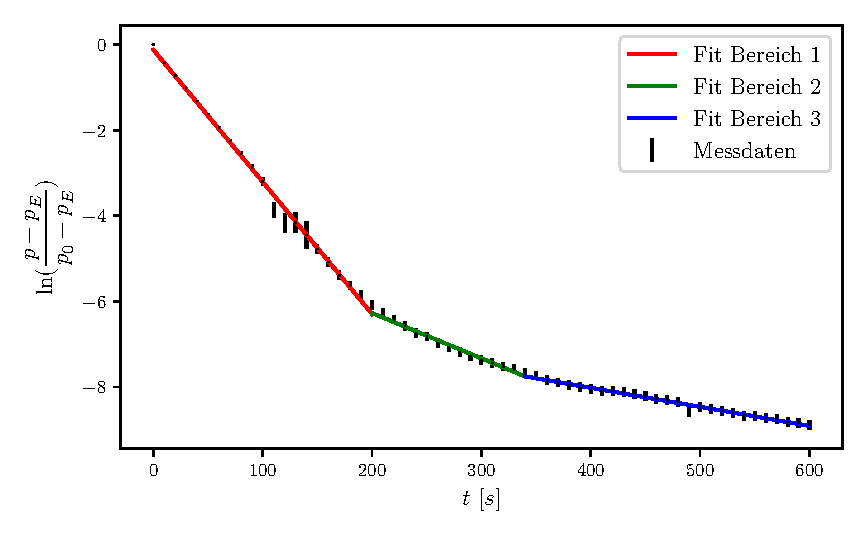
\includegraphics{build/plots/plot_ev_dreh.pdf}
      \caption{Logarithmierte Werte mit Ausgleichsgeraden für 3 Druckbereiche zur Evakuierungsmessung der Drehschieberpumpe}
      \label{fig:plotdlog}
    \end{figure}
    \noindent
    Die Parameter der Ausgleichsrechnung und das jeweilige Saugvermögen sind in der folgenden Tabelle für die entsprechenden Druckbereiche aufgelistet.

    \begin{table}[H]
      \centering
      \small
      \label{tab:para_ev_dreh}
      \begin{tabular}{l  c c c}
       \toprule
       {Druckbereich} & $\text{m} [\si{\per\second}]$ & $\text{n}$ & $\text{S} [\si{\litre\per\second}]$ \\
       \midrule
       $\SI{998}{\milli\bar}$ bis $\SI{2.3}{\milli\bar}$ & -0.0309 \pm 0.00048 & -0.1191 \pm 0.00048 & 1.0500 \pm 0.10624\\
       $\SI{2.3}{\milli\bar}$ bis $\SI{0.52}{\milli\bar}$ &-0.0106 \pm 0.00043 & -4.1571 \pm 0.00043 & 0.3598 \pm 0.03877\\
       $\SI{0.52}{\milli\bar}$ bis $\SI{0.15}{\milli\bar}$ & -0.0045 \pm 0.00011  & -6.2388 \pm 0.00011 & 0.1514 \pm 0.01563\\
      \bottomrule
      \end{tabular}
      \caption{Parameter der Ausgleichsgeraden und Ergebnisse für das Saugvermögen für die Evakuierungsmessung zur Drehschieberpumpe}
    \end{table} 

\subsubsection{Leckratenmessungen}

In diesem Abschnitt werden analog zum Vorgehen bei der Turbopumpe die Ergebnisse der Leckratenmessungen für die Drehschieberpumpe dargestellt. Die Messungen wurden bei den Gleichgewichtsdrücken $p_g = \SI{0.5}{\milli\bar}$, $p_g = \SI{9.7}{\milli\bar}$, $p_g = \SI{50}{\milli\bar}$ und $p_g = \SI{100}{\milli\bar}$ durchgeführt. Dazu werden die Messwerte jeweils graphisch mit Ausgleichsgerade dargestellt.

\begin{table}[H]
  \centering
  \caption{Messreihen zur Leckratenmessung der Drehschieberpumpe mit $p_g = 0.5$ mbar}
  \label{tab:tabled1}
  \begin{tabular}{rllll}
    \hline
       t [s] & p1 [mbar]   & p2 [mbar]   & p3 [mbar]   &  $\bar{p}$ [mbar]             \\
    \hline
          10 & 1.90 \pm 0.19 & 1.90 \pm 0.19 & 1.90 \pm 0.19 & 1.90 \pm 0.19 \\
          20 & 2.00 \pm 0.20 & 2.00 \pm 0.20 & 2.00 \pm 0.20 & 2.00 \pm 0.20 \\
          30 & 2.10 \pm 0.21 & 2.10 \pm 0.21 & 2.10 \pm 0.21 & 2.10 \pm 0.21 \\
          40 & 2.20 \pm 0.22 & 2.20 \pm 0.22 & 2.20 \pm 0.22 & 2.20 \pm 0.22 \\
          50 & 2.30 \pm 0.23 & 2.30 \pm 0.23 & 2.30 \pm 0.23 & 2.30 \pm 0.23 \\
          60 & 2.50 \pm 0.25 & 2.50 \pm 0.25 & 2.50 \pm 0.25 & 2.50 \pm 0.25 \\
          70 & 2.60 \pm 0.26 & 2.60 \pm 0.26 & 2.60 \pm 0.26 & 2.60 \pm 0.26 \\
          80 & 2.70 \pm 0.27 & 2.70 \pm 0.27 & 2.70 \pm 0.27 & 2.70 \pm 0.27 \\
          90 & 2.80 \pm 0.28 & 2.80 \pm 0.28 & 2.80 \pm 0.28 & 2.80 \pm 0.28 \\
         100 & 2.90 \pm 0.29 & 2.90 \pm 0.29 & 2.90 \pm 0.29 & 2.90 \pm 0.29 \\
         110 & 3.00 \pm 0.30 & 3.00 \pm 0.30 & 3.00 \pm 0.30 & 3.00 \pm 0.30 \\
         120 & 3.10 \pm 0.31 & 3.10 \pm 0.31 & 3.10 \pm 0.31 & 3.10 \pm 0.31 \\
         130 & 3.20 \pm 0.32 & 3.20 \pm 0.32 & 3.20 \pm 0.32 & 3.20 \pm 0.32 \\
         140 & 3.30 \pm 0.33 & 3.30 \pm 0.33 & 3.30 \pm 0.33 & 3.30 \pm 0.33 \\
         150 & 3.50 \pm 0.35 & 3.50 \pm 0.35 & 3.50 \pm 0.35 & 3.50 \pm 0.35 \\
         160 & 3.6 \pm 0.4   & 3.6 \pm 0.4   & 3.6 \pm 0.4   & 3.6 \pm 0.4   \\
         170 & 3.7 \pm 0.4   & 3.8 \pm 0.4   & 3.7 \pm 0.4   & 3.7 \pm 0.4   \\
         180 & 3.8 \pm 0.4   & 3.8 \pm 0.4   & 3.8 \pm 0.4   & 3.8 \pm 0.4   \\
         190 & 4.0 \pm 0.4   & 4.0 \pm 0.4   & 4.0 \pm 0.4   & 4.0 \pm 0.4   \\
         200 & 4.1 \pm 0.4   & 4.1 \pm 0.4   & 4.1 \pm 0.4   & 4.1 \pm 0.4   \\
    \hline
    \end{tabular}
  \end{table}

  \begin{figure}[H]
    \centering
    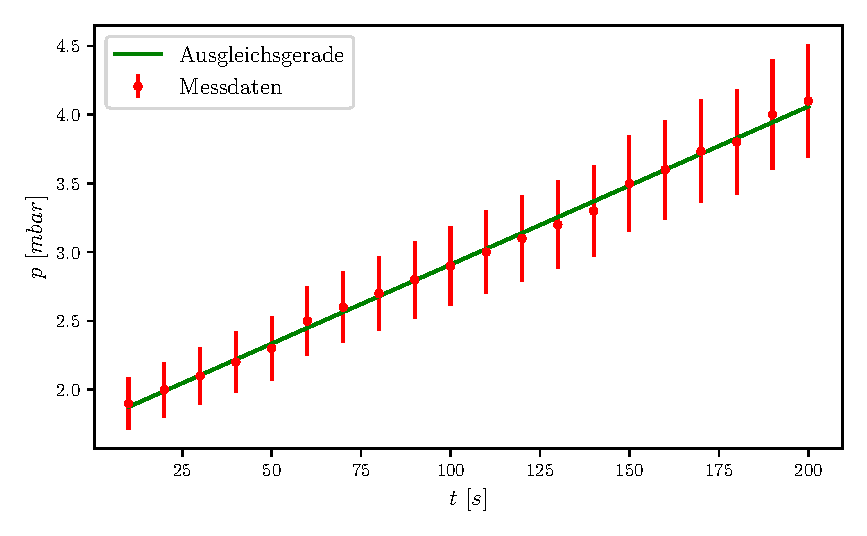
\includegraphics{build/plots/leck_dreh_0.5.pdf}
    \caption{Messwerte mit Ausgleichsgerade zur Leckratenmessung der Drehschieberpumpe bei $p_g = \SI{0.5}{\milli\bar}$}
    \label{fig:plotd1}
  \end{figure}

  \begin{table}[H]
    \centering
    \caption{Messreihen zur Leckratenmessung der Drehschieberpumpe mit $p_g = 9.7$ mbar}
    \label{tab:tabled2}
    \begin{tabular}{rllll}
      \hline
         t [s] & p1 [mbar]   & p2 [mbar]   & p3 [mbar]   &  $\bar{p}$ [mbar]        \\
      \hline
            10 & 19 \pm 4      & 19 \pm 4      & 19 \pm 4      & 19 \pm 4 \\
            20 & 23 \pm 4      & 22 \pm 4      & 22 \pm 4      & 22 \pm 4 \\
            30 & 26 \pm 4      & 26 \pm 4      & 26 \pm 4      & 26 \pm 4 \\
            40 & 30 \pm 4      & 29 \pm 4      & 29 \pm 4      & 29 \pm 4 \\
            50 & 33 \pm 4      & 33 \pm 4      & 33 \pm 4      & 33 \pm 4 \\
            60 & 37 \pm 4      & 37 \pm 4      & 36 \pm 4      & 37 \pm 4 \\
            70 & 40 \pm 4      & 40 \pm 4      & 40 \pm 4      & 40 \pm 4 \\
            80 & 44 \pm 4      & 44 \pm 4      & 44 \pm 4      & 44 \pm 4 \\
            90 & 47 \pm 4      & 47 \pm 4      & 47 \pm 4      & 47 \pm 4 \\
           100 & 51 \pm 4      & 51 \pm 4      & 51 \pm 4      & 51 \pm 4 \\
           110 & 54 \pm 4      & 54 \pm 4      & 54 \pm 4      & 54 \pm 4 \\
           120 & 58 \pm 4      & 58 \pm 4      & 58 \pm 4      & 58 \pm 4 \\
           130 & 61 \pm 4      & 61 \pm 4      & 62 \pm 4      & 61 \pm 4 \\
           140 & 65 \pm 4      & 65 \pm 4      & 65 \pm 4      & 65 \pm 4 \\
           150 & 68 \pm 4      & 68 \pm 4      & 68 \pm 4      & 68 \pm 4 \\
           160 & 72 \pm 4      & 72 \pm 4      & 72 \pm 4      & 72 \pm 4 \\
           170 & 75 \pm 4      & 75 \pm 4      & 75 \pm 4      & 75 \pm 4 \\
           180 & 79 \pm 4      & 79 \pm 4      & 79 \pm 4      & 79 \pm 4 \\
           190 & 82 \pm 4      & 82 \pm 4      & 82 \pm 4      & 82 \pm 4 \\
           200 & 86 \pm 4      & 86 \pm 4      & 86 \pm 4      & 86 \pm 4 \\
      \hline
      \end{tabular}
    \end{table}

    \begin{figure}[H]
      \centering
      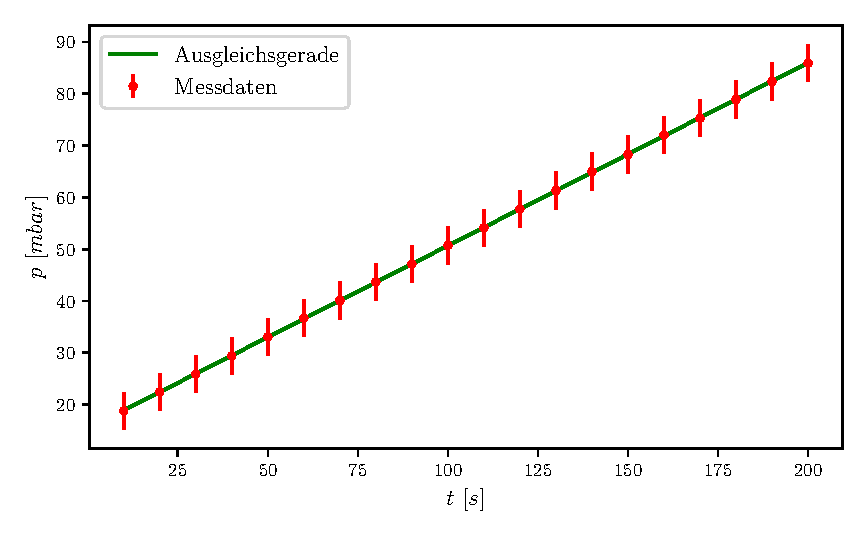
\includegraphics{build/plots/leck_dreh_9.7.pdf}
      \caption{Messwerte mit Ausgleichsgerade zur Leckratenmessung der Drehschieberpumpe bei $p_g = \SI{9.7}{\milli\bar}$}
      \label{fig:plotd2}
    \end{figure}

    \begin{table}[H]
      \centering
      \caption{Messreihen zur Leckratenmessung der Drehschieberpumpe mit $p_g = 50$ mbar}
      \label{tab:tabled3}
      \begin{tabular}{rllll}
        \hline
           t [s] & p1 [mbar]   & p2 [mbar]   & p3 [mbar]   &  $\bar{p}$ [mbar]         \\
        \hline
              10 & 76 \pm 4      & 76 \pm 4      & 75 \pm 4      & 76 \pm 4  \\
              20 & 94 \pm 4      & 94 \pm 4      & 93 \pm 4      & 93 \pm 4  \\
              30 & 111 \pm 4     & 111 \pm 4     & 110 \pm 4     & 111 \pm 4 \\
              40 & 128 \pm 4     & 128 \pm 4     & 128 \pm 4     & 128 \pm 4 \\
              50 & 146 \pm 4     & 146 \pm 4     & 145 \pm 4     & 146 \pm 4 \\
              60 & 163 \pm 4     & 163 \pm 4     & 162 \pm 4     & 163 \pm 4 \\
              70 & 181 \pm 4     & 180 \pm 4     & 180 \pm 4     & 180 \pm 4 \\
              80 & 198 \pm 4     & 198 \pm 4     & 197 \pm 4     & 198 \pm 4 \\
              90 & 214 \pm 4     & 214 \pm 4     & 213 \pm 4     & 214 \pm 4 \\
             100 & 232 \pm 4     & 232 \pm 4     & 233 \pm 4     & 232 \pm 4 \\
             110 & 249 \pm 4     & 249 \pm 4     & 248 \pm 4     & 249 \pm 4 \\
             120 & 267 \pm 4     & 266 \pm 4     & 266 \pm 4     & 266 \pm 4 \\
             130 & 284 \pm 4     & 284 \pm 4     & 283 \pm 4     & 284 \pm 4 \\
             140 & 302 \pm 4     & 301 \pm 4     & 300 \pm 4     & 301 \pm 4 \\
             150 & 319 \pm 4     & 318 \pm 4     & 318 \pm 4     & 318 \pm 4 \\
             160 & 336 \pm 4     & 336 \pm 4     & 335 \pm 4     & 336 \pm 4 \\
             170 & 354 \pm 4     & 353 \pm 4     & 352 \pm 4     & 353 \pm 4 \\
             180 & 371 \pm 4     & 371 \pm 4     & 370 \pm 4     & 371 \pm 4 \\
             190 & 388 \pm 4     & 388 \pm 4     & 387 \pm 4     & 388 \pm 4 \\
             200 & 406 \pm 4     & 405 \pm 4     & 404 \pm 4     & 405 \pm 4 \\
        \hline
        \end{tabular}
    \end{table}

    \begin{figure}[H]
      \centering
      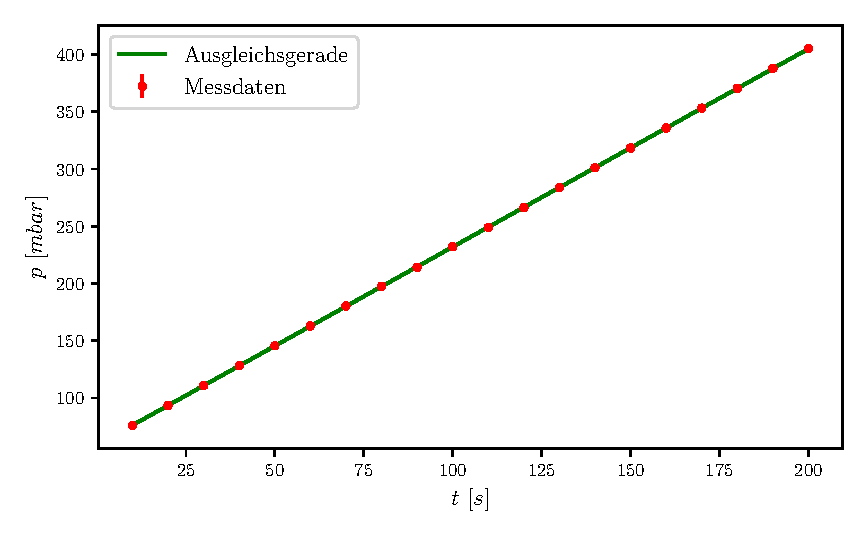
\includegraphics{build/plots/leck_dreh_50.pdf}
      \caption{Messwerte mit Ausgleichsgerade zur Leckratenmessung der Drehschieberpumpe bei $p_g = \SI{50}{\milli\bar}$}
      \label{fig:plotd3}
    \end{figure}

      \begin{table}[H]
        \centering
        \caption{Messreihen zur Leckratenmessung der Drehschieberpumpe mit $p_g = 100$ mbar}
        \label{tab:tabled4}
        \begin{tabular}{rllll}
          \hline
             t [s] & p1 [mbar]         & p2 [mbar]         & p3 [mbar]         & $\bar{p}$ [mbar]     \\
          \hline
          10 & 145 \pm 4     & 144 \pm 4     & 145 \pm 4     & 145 \pm 4 \\
          20 & 179 \pm 4     & 178 \pm 4     & 179 \pm 4     & 179 \pm 4 \\
          30 & 211 \pm 4     & 214 \pm 4     & 211 \pm 4     & 212 \pm 4 \\
          40 & 248 \pm 4     & 248 \pm 4     & 248 \pm 4     & 248 \pm 4 \\
          50 & 279 \pm 4     & 281 \pm 4     & 278 \pm 4     & 279 \pm 4 \\
          60 & 312 \pm 4     & 315 \pm 4     & 312 \pm 4     & 313 \pm 4 \\
          70 & 346 \pm 4     & 349 \pm 4     & 346 \pm 4     & 347 \pm 4 \\
          80 & 383 \pm 4     & 382 \pm 4     & 383 \pm 4     & 383 \pm 4 \\
          90 & 413 \pm 4     & 416 \pm 4     & 416 \pm 4     & 415 \pm 4 \\
         100 & 446 \pm 4     & 449 \pm 4     & 446 \pm 4     & 447 \pm 4 \\
         110 & 482 \pm 4     & 482 \pm 4     & 479 \pm 4     & 481 \pm 4 \\
         120 & 515 \pm 4     & 514 \pm 4     & 512 \pm 4     & 514 \pm 4 \\
         130 & 544 \pm 4     & 546 \pm 4     & 544 \pm 4     & 545 \pm 4 \\
         140 & 576 \pm 4     & 578 \pm 4     & 575 \pm 4     & 576 \pm 4 \\
         150 & 610 \pm 4     & 609 \pm 4     & 606 \pm 4     & 608 \pm 4 \\
         160 & 640 \pm 4     & 639 \pm 4     & 636 \pm 4     & 638 \pm 4 \\
         170 & 666 \pm 4     & 668 \pm 4     & 666 \pm 4     & 667 \pm 4 \\
         180 & 698 \pm 4     & 697 \pm 4     & 695 \pm 4     & 697 \pm 4 \\
         190 & 723 \pm 4     & 722 \pm 4     & 725 \pm 4     & 723 \pm 4 \\
         200 & 750 \pm 4     & 751 \pm 4     & 749 \pm 4     & 750 \pm 4 \\
        \hline
      \end{tabular}
      \end{table}

      \begin{figure}[H]
        \centering
        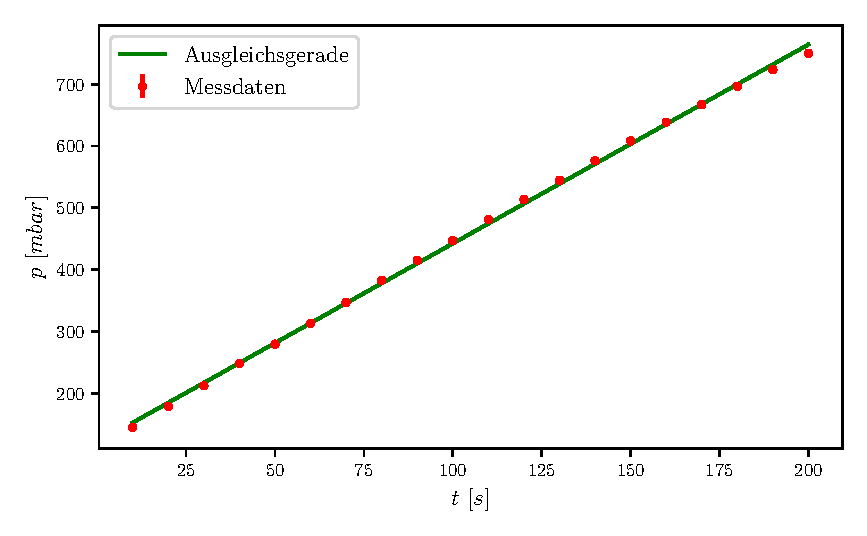
\includegraphics{build/plots/leck_dreh_100.pdf}
        \caption{Messwerte mit Ausgleichsgerade zur Leckratenmessung der Drehschieberpumpe bei $p_g = \SI{100}{\milli\bar}$}
        \label{fig:plotd4}
      \end{figure}
\noindent
Auch für die Drehschieberpumpe lässt sich aus den Parametern der Ausgleichsgeraden die Saugleistung bestimmen:
      \begin{table}[H]
        \centering
        \small
      \label{tab:para_leck_dreh}
      \begin{tabular}{l  c c c}
       \toprule
       $p_g [\si{\milli\bar}]$ & $\text{m} [\si{\per\second}]$ & $\text{n}$ & $\text{S} [\si{\litre\per\second}]$ \\
       \midrule
       $\SI{0.5}{\milli\bar}$ & 0.0115 \pm 0.000138 & 1.759 \pm 0.000138 & 0.782 \pm 0.0788\\
       $\SI{9.7}{\milli\bar}$ &0.353 \pm 0.000372 & 15.374 \pm 0.000372 & 1.237 \pm 0.124\\
       $\SI{50}{\milli\bar}$ & 1.731 \pm 0.000889  & 58.788 \pm 0.000889 & 1.1773 \pm 0.118\\
       $\SI{100}{\milli\bar}$ & 3.220 \pm 0.0235  & 120.251 \pm 0.0235 & 1.0947 \pm 0.1010\\
      \bottomrule
      \end{tabular}
      \caption{Parameter der Ausgleichsgeraden und Ergebnisse für das Saugvermögen zur Leckratenmessung der Drehschieberpumpe für unterschiedliche Gleichgewichtsdrücke}
    \end{table} 